%
% Optional reading
%

\begin{frame}[plain,c]
\begin{center}
{\Huge \bf Optional reading for Lecture \thislecture}
\end{center}
\end{frame}

% ------------------------------------------------------------------------------

%
% Worked example :
%

{
\problemslide

\begin{frame}{Worked example: Electric field and force of 3 point charges}

\begin{blockexmplque}{Question}
  Three charges are arranged as following:
  $Q_1$ = 1 nC at (-1,-1,0) cm, $Q_2$ = 1 nC at (1,-1,0) cm and $Q_3$ = -2nC at (0,2,0) cm.
  Calculate:
  \begin{enumerate}
    \item The electric field (vector) at the point (0,0,0).
    \item The force acting on charge $Q_3$.
  \end{enumerate}
\end{blockexmplque}

\vspace{0.2cm}

The electric field $\vec{E}$ at $\vec{r}$, due to $Q_1$, $Q_2$, and $Q_3$,
is given by the superposition of the fields produced by each point charge:
\begin{equation*}
  \vec{E}(\vec{r}) = \frac{1}{4\pi \epsilon_0}
       \sum_{i=1}^{2} \frac{Q_i}{|\vec{r}-\vec{r}_i|^3} \Big( \vec{r}-\vec{r}_i \Big)
\end{equation*}

Therefore, at $\vec{r}=\vec{0}$, it is given by:
\begin{equation*}
  \vec{E}(\vec{0}) = \frac{1}{4\pi \epsilon_0} \Big\{
          \frac{Q_1}{|\vec{r}_1|^3} \Big( - \vec{r}_1 \Big) +
          \frac{Q_2}{|\vec{r}_2|^3} \Big( - \vec{r}_2 \Big) +
          \frac{Q_3}{|\vec{r}_3|^3} \Big( - \vec{r}_3 \Big)
      \Big\}
\end{equation*}

\end{frame}

%
%
%

\begin{frame}{Worked example: Electric field and force of 3 point charges}

Substituting the given quantities into the previous equation, we get:
\begin{equation*}
  \vec{E}(\vec{0}) =
      (9.0 \times 10^9 \; \frac{N \cdot m^2}{C^2}) \Big\{
          \frac{ (1.0 \times 10^{-9} \; C)}{\sqrt{2}^3 \times 10^{-6} \; m^3} \Big( 1, 1, 0 \Big) \times 10^{-2} m +
\end{equation*}
\begin{equation*}
        + \frac{ (1.0 \times 10^{-9} \; C)}{\sqrt{2}^3 \times 10^{-6} \; m^3} \Big(-1, 1, 0 \Big) \times 10^{-2} m +
          \frac{(-2.0 \times 10^{-9} \; C)}{2^3 \times 10^{-6} \; m^3}        \Big( 0,-2, 0 \Big) \times 10^{-2} m
      \Big\} \Rightarrow
\end{equation*}

\begin{equation*}
  \vec{E}(\vec{0}) =
      9.0 \times 10^9 \Big\{
          \frac{2.0 \times 10^{-11}}{\sqrt{2}^3 \times 10^{-6}} + \frac{4.0 \times 10^{-11}}{2^3 \times 10^{-6}} \Big\} \Big(0, 1, 0 \Big) \; \frac{N}{C}
  \Rightarrow
\end{equation*}

\begin{equation*}
  \vec{E}(\vec{0}) =
      9.0 \times 10^9 \Big\{
               0.707 \times 10^{-5} + 0.500 \times 10^{-5} \Big\} \Big(0, 1, 0 \Big) \; \frac{N}{C}
  \Rightarrow
\end{equation*}

\begin{equation*}
  \vec{E}(\vec{0}) =
      1.0863 \times 10^5 \Big(0, 1, 0 \Big) \; \frac{N}{C}
\end{equation*}

\end{frame}

%
%
%

\begin{frame}{Worked example: Electric field and force of 3 point charges}


The force $\vec{F}_{3}$ acting on $Q_3$ is the vector sum of $\vec{F}_{31}$ and $\vec{F}_{32}$.

\begin{equation*}
  \vec{F}_{31} = \frac{1}{4\pi \epsilon_0} \frac{Q_1 Q_3}{|\vec{r}_3-\vec{r}_1|^3} \Big( \vec{r}_3-\vec{r}_1 \Big) \Rightarrow
\end{equation*}
\begin{equation*}
  \vec{F}_{31} = (9.0 \times 10^9 \; \frac{N \cdot m^2}{C^2})
     \frac{(1.0 \times 10^{-9} \; C)(-2.0 \times 10^{-9} \; C)}{\sqrt{10.0}^3 \times 10^{-6} \; m^3} \Big(1,3,0\Big) \times 10^{-2} \; m
\end{equation*}

\begin{equation*}
  \vec{F}_{32} = \frac{1}{4\pi \epsilon_0} \frac{Q_2 Q_3}{|\vec{r}_3-\vec{r}_2|^3} \Big( \vec{r}_3-\vec{r}_2 \Big) \Rightarrow
\end{equation*}
\begin{equation*}
  \vec{F}_{32} = (9.0 \times 10^9 \; \frac{N \cdot m^2}{C^2})
     \frac{(1.0 \times 10^{-9} \; C)(-2.0 \times 10^{-9} \; C)}{\sqrt{10.0}^3 \times 10^{-6} \; m^3} \Big(-1,3,0\Big) \times 10^{-2} \; m
\end{equation*}

\begin{equation*}
  \vec{F}_3 =
  \vec{F}_{31} + \vec{F}_{32} = (9.0 \times 10^9 \; \frac{N \cdot m^2}{C^2})
     \frac{(-2.0 \times 10^{-18} \; C^2)}{\sqrt{10.0}^3 \times 10^{-6} \; m^3} \Big(0,6,0\Big) \times 10^{-2} \; m \Rightarrow
\end{equation*}

\begin{equation*}
  \vec{F}_{3} = -34.1 \Big(0,1,0\Big) \; {\mu}N
\end{equation*}

\end{frame}

} %\problemslide


% ------------------------------------------------------------------------------

%
% Worked example :
%

{
\problemslide

\begin{frame}{Worked example: Electric field and force of 3 point charges}

\begin{blockexmplque}{Question}
  In the figure below, particle 1 of charge +1.0 $\mu$C and particle 2
  of charge -3.0 $\mu$C are held at separation $L$ = 10.0 cm on an x axis.
  If particle 3 of unknown charge $q_3$ is to be located such that the net
  electrostatic force on it from particles 1 and 2 is zero,
  what must be the x and y coordinates of particle 3?
  \begin{center}
      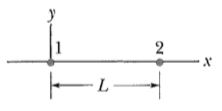
\includegraphics[width=0.30\textwidth]{./images/problems/lect01_3charges_0_net_force_on_third.png}
  \end{center}
\end{blockexmplque}

\vspace{0.2cm}

There is no equilibrium position for $q_3$ between the two fixed charges,
because it is being pulled by one and pushed by the other
(since $q_1$ and $q_2$ have different signs).
In this region, the two forces on q3 ($\vec{F}_{31}$ and $\vec{F}_{32}$)
have components that cannot cancel.

\end{frame}

%
%
%

\begin{frame}{Worked example: Electric field and force of 3 point charges}

  For the same reason, there are no equilibrium positions off-axis
  (with the axis defined as that which passes through the two fixed charges),
  and therefore y=0.\\
  \vspace{0.3cm}

  On the semi-infinite region of the axis that is nearest $q_2$
  and furthest from $q_1$ an equilibrium position for $q_3$ cannot be found
  because $|q_1| < |q_2|$ and the magnitude of force exerted by $q_2$
  is everywhere (in that region) stronger than that exerted by $q_1$ on $q_3$.\\
  \vspace{0.3cm}

  Thus, we must look in the semi-infinite region of the axis which is nearest
  $q_1$ and furthest from $q_2$ (x$<$0).

\end{frame}

%
%
%

\begin{frame}{Worked example: Electric field and force of 3 point charges}

  In that region, the net force on $q_3$ has magnitude which is given by:
  \begin{equation*}
     F_{3} = \left\rvert
               \frac{1}{4\pi\epsilon_0} \frac{|q_1 q_3|}{|x|^2} -
               \frac{1}{4\pi\epsilon_0} \frac{|q_2 q_3|}{(L+|x|)^2}
              \right\rvert
  \end{equation*}

  Setting $F_{3}$ equal to zero, the above expression yields:
  \begin{equation*}
    \frac{|q_1|}{|x|^2} - \frac{|q_2|}{(L+|x|)^2} = 0 \Rightarrow
    \Big(\frac{L+|x|}{|x|} \Big)^{2} = \frac{|q_2|}{|q_1|} \Rightarrow
    \frac{L}{|x|} + 1 = \sqrt{\frac{|q_2|}{|q_1|}} \Rightarrow
  \end{equation*}

  \begin{equation*}
    |x| = \frac{L}{\sqrt{\frac{|q_2|}{|q_1|}} - 1} \Rightarrow
  \end{equation*}

  \begin{equation*}
    |x| = \frac{10\;cm}{\sqrt{\frac{|-3\;{\mu}C|}{|+1\;{\mu}C|}} - 1}
        = \frac{10\;cm}{\sqrt{3} - 1} \approx 13.66 \; cm
    \Rightarrow x = -13.66 \; cm
  \end{equation*}

\end{frame}

} %\problemslide

% ------------------------------------------------------------------------------

%
% Programming
%

{
\programmingslide

%
%
%

\begin{frame}{PHYS201 scientific programming task for Lecture \thislecture}

{\small

Write a program that:
\begin{itemize}
{\scriptsize
  \item {\bf Can read an arbitrary distribution of N discrete charges (in 2-D)},\\
        e.g. by accepting as input a text file with N rows, where the $i^{th}$
        row contains the coordinates $x_i$, $y_i$ in m, and the charge $q_i$ in C.
  \item {\bf Allows you to visualise the input charge distribution},\\
        e.g using appropriately-positioned circles whose color or size represents amount of charge.
  \item {\bf Allows you to visualise the electric field lines}
        in the vicinity of the charge distrubution.\\
}
\end{itemize}

\vspace{0.2cm}
Test you program, reproducing some of the simpler field maps shown before.\\

\vspace{0.2cm}
Document your program, upload it to a GitHub repository, and send me a link!\\

}

\end{frame}


} % programming
